\documentclass[Lecture.tex]{subfiles}
\begin{document}
\section{1.2: Linear Functions}

\begin{frame}{Definition}
  \begin{defn}
    A function, $f$, is {\it linear} if there exist real numbers $m$ and $b$ such that
    $$f(x) = mx + b.$$
    \begin{itemize}
    \item<2->
      Linear functions have domain and range $\R$,
    \item<3->
      The number $m$ is called the {\it slope} of the $f$,
    \item<4->
      The number $b$ is the $y$-intercept,
    \item<5->
      This form is usually called the {\it Slope-Intercept Form} of a line.
    \end{itemize}
  \end{defn}
\end{frame}

\begin{frame}{Graph of a Linear Function}
  The graph of $f(x) = mx + b$ is always a line.
  \pause
  They come in three flavors:
  \begin{itemize}
  \item<3->
    Increasing ($0 < m$):
    \begin{center}
      \begin{tikzpicture}
        \draw (0,0) -- (1,1);
      \end{tikzpicture}
    \end{center}
  \item<4->
    Decreasing ($m < 0$):
    \begin{center}
      \begin{tikzpicture}
        \draw (0,0) -- (1,-1);
      \end{tikzpicture}
    \end{center}
  \item<5->
    Horizontal ($m = 0$):
    \begin{center}
      \begin{tikzpicture}
        \draw (0,0) -- (1,0);
      \end{tikzpicture}
    \end{center}
  \end{itemize}
  
\end{frame}

\begin{frame}{Point-Slope Form}
  \begin{defn}
    Given: 
    \begin{itemize}
    \item<2->
      a point, $(x_0, y_0)$,
    \item<3->
      a slope, $m$,
    \end{itemize}
    \onslide<4->{
      the equation of the line through $(x_0,y_0)$ with slope $m$ is
      $$y - y_0 = m(x - x_0).$$
    }
  \end{defn}
\end{frame}

\begin{frame}{Two Points Determine a Line}
  Given two points, $(x_0, y_0)$ and $(x_1, y_1)$, the slope of the line passing through them is
  $$m = \frac{y_0 - y_1}{x_0 - x_1} = \frac{y_1 - y_0}{x_1 - x_0}.$$\\
  \pause
  The line passing through these two points is
  $$ y - y_0 = m(x - x_0)\ \text{or}\ y - y_1 = m(x - x_1).$$
  \pause
  To see these are the same line, put them both into Slope-Intercept Form.
\end{frame}

\begin{frame}{Two Points Determine a Line (Cont.)}
  \begin{eqnarray*}
    \onslide<1->{y &=& mx - \frac{y_0 - y_1}{x_0 - x_1}x_0 + y_0\\}
    \onslide<2->{&=& mx + \frac{(y_1 - y_0)x_0 + (x_0 - x_1)y_0}{x_0 - x_1}\\}
    \onslide<3->{&=& mx - \frac{x_0y_1 - x_1y_0}{x_0 - x_1}}
  \end{eqnarray*}
  \begin{eqnarray*}
    \onslide<1->{y &=& mx - \frac{y_0 - y_1}{x_0 - x_1} x_1 + y_1\\}
    \onslide<2->{&=& mx + \frac{(y_1 - y_0)x_1 + (x_0 - x_1)y_1}{x_0 - x_1}\\}
    \onslide<3->{&=& mx + \frac{x_0y_1 - x_1y_0}{x_0 - y_0}}
  \end{eqnarray*}
\end{frame}

\begin{frame}{Difference Quotients}
  \begin{defn}
    Let $f$ be a function.
    \onslide<2->{
      Given $x_0$, $x_1$ in the domain of $f$}\onslide<3->{, the {\it difference quotient} is
      $$\frac{f(x_1) - f(x_0)}{x_1 - x_0} = \frac{f(x_0) - f(x_1)}{x_0 - x_1}$$
    }
    \onslide<4->{
      This is just the slope of the line through $(x_0, f(x_0))$ and $(x_1, f(x_1))$.}
    \onslide<5->{
      This line is usually called the {\it Secant Line}}.
  \end{defn}
\end{frame}

\begin{frame}{Difference Quotients for Linear Functions}
  Let $f(x) = mx + b$.
  \onslide<2->{
    Given $x_0$ and $x_1$:
  }
  \begin{eqnarray*}
    \onslide<3->{\frac{f(x_1) - f(x_0)}{x_1 - x_0} &=& \frac{mx_1 + b - (mx_0 + b)}{x_1 - x_0}\\}
    \onslide<4->{&=& \frac{mx_1 - mx_0 + b - b}{x_1 - x_0}\\}
    \onslide<5->{&=& \frac{m(x_1 - x_0)}{x_1 - x_0}\\}
    \onslide<6->{&=& m}
  \end{eqnarray*}
  \onslide<7->{Hence for a linear function, the difference quotient is just the slope.}
\end{frame}

\begin{frame}{Difference Quotients for Non-Linear Functions}
  Let $f(x) = x^2$. For $x_0 = -1$, $x_1 = 2$:
  $$\onslide<2->{\frac{f(-1) - f(2)}{-1 - 2}} \onslide<3->{= \frac{(-1)^2 - 2^2}{-3}} \onslide<4->{= \frac{1 - 4}{-3}} \onslide<5->{= \frac{-3}{-3} = 1.}$$
  \onslide<6->{This is the slope of the secant line:}
  \begin{center}
    \onslide<6->{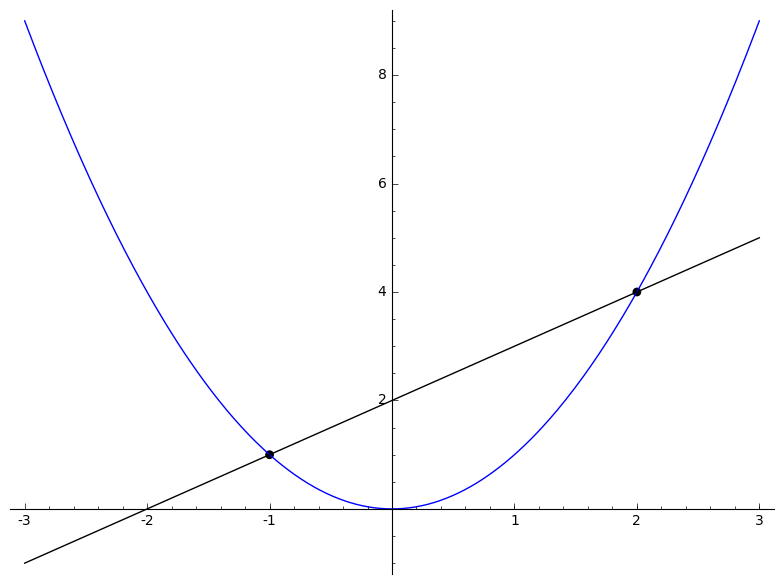
\includegraphics[scale=0.25]{diffQuo1}}
  \end{center}
\end{frame}

\begin{frame}{Difference Quotients for Non-Linear Functions (Cont.)}
  \onslide<1->{For $x_0 = 0$, $x_1 = 2$:}
  $$\onslide<2->{\frac{f(0) - f(2)}{0 - 2}} \onslide<3->{= \frac{0 - 4}{-2}} \onslide<4->{= \frac{4}{2} = 2.}$$
  \onslide<5->{This is the slope of the secant line:}
  \begin{center}
    \onslide<5->{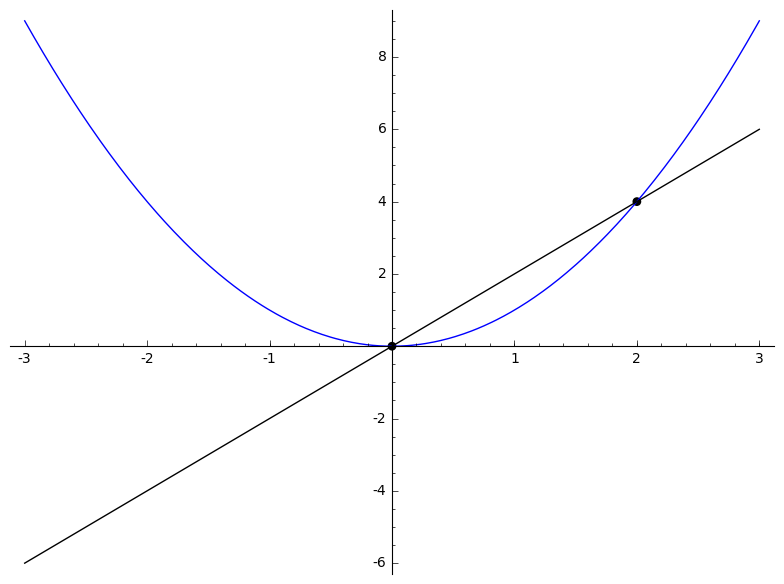
\includegraphics[scale=0.25]{diffQuo2}}
  \end{center}
\end{frame}
\end{document}
